\documentclass{template}
\usepackage{graphicx,parskip,appendix,float}
\usepackage[ruled] {algorithm2e}
\usepackage{url,amsmath,amssymb,fancybox,listings,pdfpages,caption,multicol,datetime,rotating,booktabs,dsfont,mathtools,textcomp}
%\usepackage[usenames,dvipsnames]{color}
\usepackage[pagebackref=false,pdffitwindow=true]{hyperref}
\usepackage{csquotes}
\usepackage{physics}
\usepackage[style=authoryear,backend=biber]{biblatex}
\addbibresource{thesis.bib}

%NOTE: The hyperref usepackage should be the last \usepackage!!
%NOTE: When pagebackref=true an error will appear at the end of compiling. press `q' to ignore
%NOTE: Referencing Algorithms does not work if this usepackage is before the hyperref include.!!
%NOTE: This is a comment, ignored when the document is compiled
%NOTE: The following document configuration settings generally do not need to be modified
%NOTE: More packages may need to be added to provide additional functionality

\hypersetup{
    pdftitle    = {Report Title},
    pdfauthor   = {Author Name},
    pdfsubject  = {Subject Area},
    pdfkeywords = {Comma separated list of keywords},
    colorlinks  = true, anchorcolor = blue, filecolor = blue, urlcolor = blue,
    linkcolor   = blue,    %NOTE: change (blue) to (colIdentifier) to have links within the document in Black
    citecolor   = blue,    %NOTE: change (blue) to (colIdentifier) to have citation links within the document in Black
}

\definecolor{colBackGrnd}{rgb}{1,1,0.8}
\definecolor{colKeys}{rgb}{0,0,1}
\definecolor{colIdentifier}{rgb}{0,0,0}
\definecolor{colComments}{rgb}{0,.5,0}
\definecolor{colString}{rgb}{0,0,1}
\definecolor{colWhite}{rgb}{1,1,1}

\newcommand{\MyHookSign}{\hbox{\ensuremath\hookleftarrow}}

\newtheorem{Theorem}{Theorem}
\newtheorem{Proposition}[Theorem]{Proposition}
\newtheorem{Lemma}[Theorem]{Lemma}
\newtheorem{Proof}[Theorem]{Proof}
\newtheorem{Remark}[Theorem]{Remark}
\newtheorem{Claim}[Theorem]{Claim}
\newtheorem{Example}[Theorem]{Example}
\newtheorem{Definition}[Theorem]{Definition}

%NOTE: Setup for including program listings
\lstset{%
    float=H,
    basicstyle=\ttfamily\footnotesize,
    identifierstyle=\color{colIdentifier},
    keywordstyle=\color{colIdentifier}, %
    stringstyle=\color{colIdentifier},
    commentstyle=\color{colIdentifier}, %
    columns=flexible,
    tabsize=2,
    frame=single,
    extendedchars=true, %
    showspaces=false,
    showstringspaces=false,
    numbers=left, %
    numberstyle=\footnotesize,
    breaklines=true,
    prebreak={\space\MyHookSign},
    language=Java,
    backgroundcolor=\color{colBackGrnd},
    breakautoindent=true, %
    captionpos=b%
} %\hypersetup{colorlinks=true, citecolor=\color{colIdentifier}}

\sloppy %NOTE: To ensure the Right Hand Margin is used (Especially for long URLS)
%NOTE: END of the document configuration settings

\begin{document}

\DeclareGraphicsExtensions{.jpg,.png,.gif,.pdf}
%NOTE: When inserting Figures if the extension of the graphic file is not provided LaTeX will automatically search
% for the extensions declared above, in the order declared.

\title{\huge{Queasy/KetPsi}}
\author{Maharshi Kadeval\\Rajiv Chitale\\Rishit D\\Vedant Bhandare}
\degreetitle{Degree Title} % Replace with appropriate degree
\rpttype{BTech}    % Replace MSc with BSc for Honours Degree Year projects.
\principaladviser{Dr. Jyothi Vedurada}

\beforeabstract
\prefacesection{Abstract}


\prefacesection{Acknowledgements}


\afterpreface \afterabstract

% \listofalgorithms   %NOTE: Will generate a list of Algorithms in the Table of Contents Section
% \lstlistoflistings  %NOTE: Will generate a list of Program Listings in the Table of Contents Section

%NOTE: Include the relative reference for each chapter to be included
% dividing the thesis file structure into a number of directories aids development
% format: directoryName/filename (the .tex extension is not required for the filename)

\chapter{Introduction}
\pagenumbering{arabic} \setcounter{page}{1}

A short paragraph introducing the topic the chapter examines.


\section{Background}

A number of pages about the background of the project.

\section{About this Thesis}
This is the thesis of \emph{Insert Full Name Here}, submitted as part of the requirements for the degree of MSc Computing: Software Technology at the School of Computing, Robert Gordon University, Scotland.

A number of paragraphs detailing the main expectations of this body of work.


\section{Chapter List}
Provide a list of all the chapters within the thesis and a brief summary of the content.

\textbf{Chapter \ref{ch:Background}} Background Research. This chapter
deals with $\ldots$.

\textbf{Chapter \ref{ch:Design}} Design. This chapter
deals with $\ldots$.

\textbf{Chapter \ref{ch:Implementation}} Implementation. This chapter
deals with $\ldots$.

\textbf{Chapter \ref{ch:Evaluation}} Evaluation \& Testing. This chapter
deals with $\ldots$.

\textbf{Chapter \ref{ch:Conclusion}} Conclusion. The conclusions of the thesis are presented.

\textbf{Chapter \ref{ch:usingLatex}} Using \LaTeX. This chapter
deals with how to use the \LaTeX \space system. \textcolor{red}{ERASE THIS LINE ONCE YOU ARE DONE!}


\section{Conclusion}
A short conclusion summarising the chapter.
\chapter{Background Research}\label{ch:Background}

This chapter provides some background research on the project and examines some previous work.

\section{Conclusions}

The main conclusions for this chapter.



\chapter{Structure}\label{ch:struct}


\section{\texttt{init} Section}
This section contains three necessary statements that provide the compiler with necessary information about qbits
\begin{lstlisting}
        #registers quantum = 3
        #registers classical = 2
        #iters = 1000
\end{lstlisting}
to set number of quantum registers, set number of classical registers and set number of iterations, respectively. \\

Optional statements include initializing states of quantum registers:
\begin{lstlisting}
    #set quantum states -> (2,3), (0,1), (5,5)
    #set classical states -> 0, 1
\end{lstlisting}
This sets the state of first quantum register as $2+3i$, second one as $i$ and third one as $5+5i$ and sets the state of first classical register as 0 and second one as 1.\\

This section will also have user defined code block definitions (refer to block definitions section)
\begin{lstlisting}                                                                                                                                                                             
    block (i,j,k) -> (p,q,r) {                                                                                                                                                                 
        $                                                                                                                                                                                      
            statement calls                                                                                                                                                                    
        $                                                                                                                                                                                      
    }                                                                                                                                                                                          
\end{lstlisting}                                                                                                                                                                               
                                                                                                                                                                                                   
\section{\texttt{main} Section}                                                                                                                                                              
    \textbackslash begin marks the beginning of the main section and \textbackslash end marks the end of the main section. This section includes                                               
    \begin{itemize}                                                                                                                                                                            
        \item calls to pre-defined or user-defined  \emph{blocks} (refer to block definitions section)                                                                                         
        \item \textbackslash barrier: It's a directive to the compiler to not combine blocks before and after \textbackslash barrier                                                           
        \item  \emph{measure} calls block that reads the value of a register and stores it in another register (both registers provided by the programmer)                                     
        \item condition-otherwise for conditional statements                                                                                                                                   
        \item  \emph{for},  \emph{for\_lex} and \emph{for\_zip} loops for repetitive calls to blocks.                                                                                          
    \end{itemize}     
        
\section{\texttt{output} Section}
    This section contains the features of any general programming language to help interpret the results of the quantum experiment further and better understand the results from 
    repeated runs of the circuit. \\
    This section mostly contains C-like features but syntactic sugar for certain operations and loops. We also support more datatypes for vector and array manipulation.
                                                                                                                                                                                                   
                                                                                                                                                                                                   

\chapter{Lexemes}\label{ch:Lexemes}

                                                                                                                                                                                  
\section{Comments}                                                                                                                                                                  
\begin{itemize}                                                                                                                                                                                
    \item \$ \texttt{this is a valid comment} \$                                                                                                                                                        
    \item \$\\  \texttt{                                                                                                                                                                               
    this is a valid \\                                                                                                                                                                         
    multiline comment\\    }                                                                                                                                                                    
    \$                                                                                                                                                                                         
\end{itemize}                                                                                                                                                                                  

\section{Whitespaces}                                                                                                                                                                
We ignore all whitespaces in the \texttt{\textbackslash output} section; although we consider newlines in the \texttt{\textbackslash init} and \texttt{\textbackslash main} sections. 

\section{Reserved Keywords}
Some of the keywords used in the language are listed down below:
\begin{itemize}
    \item \texttt{registers}
    \item \texttt{quantum}
    \item \texttt{classical}
    \item \texttt{iters}
    \item \texttt{set}
    \item \texttt{states} 
    \item \texttt{block}
    \item \texttt{for}
    \item \texttt{for\_lex}
    \item \texttt{for\_zip}
    \item \texttt{condition}
    \item \texttt{otherwise}
    \item \texttt{begin}
    \item \texttt{end}
    \item \texttt{output}
    \item \texttt{barrier}
    \item \texttt{X}, \texttt{Y}, \texttt{Z}, \texttt{H} (gate names)
\end{itemize}

Apart from the above keywords, we also include reserved keywords for datatypes like \texttt{int}, \texttt{list}, \texttt{float}, \texttt{complex}, \texttt{matrix} etc.

\section{Punctuations}
Some of the punctuations in our language include $\left[,\right]\,\{,\},(\,)\,;,\rightarrow$.

\section{Identifiers}
We again standard conventions for identifiers; they can start with \_ or a character from the alphabet, followed by an alphanumeric sequence.

\section{Operands}
All standard operands in most common \& general programming languages are available. Apart from these operands, we also use $\rightarrow$ indicating control from one qubit to another.
Similarly, we have ternaries to indicate a Classical-Register's control over a qubit. This is illustrated in the following section.

% \include{Ops_Exp/ops}
% \include{Declarations/dec}
\chapter{Statements}\label{ch:stmt}

\subsection{Save Command}
\begin{lstlisting}
     \save filename.csv
\end{lstlisting}
This command saves the output from main section of the code into an output csv file which can be used for further data manipulation

\subsection{Echo Command}
\begin{lstlisting}
     \echo
\end{lstlisting}
This prints the output from the main section of the code to the terminal

\section{Output Statements}
This section mainly involves mainpulating the data received from the main section. These are basic arithmetic operations and also allows graphical interpretation of the data received.\\
It allows basic programming constructs any other programming language can offer:

\begin{itemize}
    \item Declaration statements
    \begin{itemize}
        \item It follows C style syntax for variable declaration.
    \end{itemize}
        
    \item Expression statements
    \begin{itemize}
        \item This may involve using variables, carrying out arithmetic operations on them and assigning to other variables. 
    \end{itemize}
    \item Conditional statements
    \begin{itemize}
        \item It follows C-style conditional statements but with a different flavour:
        \begin{lstlisting}
            condition(x > 3){
                ...    
            }
            otherwise{
                ...
            }
        \end{lstlisting}
    \end{itemize}
    \item Loop statements
    \begin{itemize}
        \item Three kinds of for loops are provided:
        \begin{itemize}
            \item for: it initializes an integer (i in this case). The integer loops through values from start to end (exclusive). The step in values can be provided optionally. These parameters are provided as a tuple. This is followed by the body of statements enclosed by curly braces.
            \begin{lstlisting}
            for i in (start:end) 
            {
                X: i 
            }
            
            for i in (start:end:step) {
                Y: i 
            }
            \end{lstlisting}
                
            \item for\_lex: loops through all permutations of multiple integers in lexicographical order, in their respective ranges
            \begin{lstlisting}
            for_lex (i,j,k) in (0:5,5:10,10:15) {
                X: i -> j
                Y: j -> k
            }
            \end{lstlisting}
            
            \item for\_zip: loops through multiple variables simultaneously. 
            \begin{lstlisting}
            for_zip (i,j) in (0:3,9:4:-2) {
                X: i -> j
            }
            \end{lstlisting}
            Here (i,j) take values (0,9), (1,7), (2,5)
        \end{itemize}
    \end{itemize}
\end{itemize}

Some additional features for data-manipulation are provided: \textbf{(more to be added on the go)}
\begin{itemize}
    \item Difference or Sum of arrays
    \begin{lstlisting}
        x = diff(A,B)
        y = sum(A,B)
    \end{lstlisting}

    \item Standard deviation of a list of numbers
    \begin{lstlisting}
        a = std_dev(A)    
    \end{lstlisting}
    
    \item Variance of a list of numbers
    \begin{lstlisting}
        a = var(A)    
    \end{lstlisting}
    
\end{itemize}

\section{Operators}
\begin{enumerate}
    \item \textbf{X}:2 - Swap operation\\
    Here 2 is the target register and X is the operand
    \item \textbf{X}: 2 $->$ 3\\  Here 2 is the control register, 3 is target register and X is the operand.
    \item All other common operands in general programming languages are also included with similar operator precedence.
\end{enumerate}


\section{Binary If}
This statement consists of a classical register and a quantum operator with a ? in between. The quantum operation only takes place if the classical register contains a 1. 
\begin{lstlisting}
    2 ? X : 4->5 
\end{lstlisting}

\section{Measure}
This reads from a quantum register (left) and stores the observation to a classical register (right). An arrow is used as punctuation. The qubit ceases to exist after this operation.
\begin{lstlisting}
    measure: 4->1
\end{lstlisting}


\section{Block}
A collection of statements can be abstracted and reused like an operation. A block is analogous to a user defined function. 

\begin{itemize}
    \item \emph{Definition}: \\
    This consists of a call signature followed by a body of statements enclosed in square braces. The block-name consists of alphanumeric characters and underscore. It must start with an uppercase letter.

    \begin{lstlisting}
    block MyBlock: (a,b,c) [
        $ statements $
    ]
    \end{lstlisting}
    A user may also define a function with an arrow operator to make the control and target registers more explicit. 
    Note that a block may contain statements other than quantum operations, such as for.
    \begin{lstlisting}
    block MyBlock_2: (i,j,k) -> (p,q) [
        for t in (i..j)
        {
            Y: t->p
            k? X: q
        }
    ]
    \end{lstlisting}

  \item \emph{Call}:
    A block operator is fed arguments similar to operands in a quantum operation.
    \begin{lstlisting}
    MyBlock_2: (2,9,0) -> (0,1)
    \end{lstlisting}
\end{itemize}
%\chapter{Design}\label{ch:Design}

This chapter examines the design of the project.

\section{Conclusions}

The main conclusions for this chapter.



%\chapter{Implementation}\label{ch:Implementation}

This chapter examines the implementation of the project.

\section{Conclusions}

The main conclusions for this chapter.



%\chapter{Evaluation \& Testing}\label{ch:Evaluation}

This chapter evaluates the overall project and provides results of tests carried out.

\section{Conclusions}

The main conclusions for this chapter.



%\chapter{Conclusion}\label{ch:Conclusion}

This chapter summarises the main outcomes and conclusions resulting from this body of work.

\section{Conclusions}

The main conclusions that may be drawn from the body of work.

\section{Future Work}

Further development that could be carried out in the future.

%\chapter{Using \LaTeX}\label{ch:usingLatex}

There are several reasons why one should prefer \LaTeX \space to a WYSIWYG word processor like Microsoft Word: \textsl{portability}, \textsl{lightness}, \textsl{security} are just a few of them (not to mention that \LaTeX \space is free). There is still a further reason that should definitely convince you to abandon MS Word for the development of a dissertation: you will never be able to produce professionally typeset and well-structured documents using most standard WYSIWYG tools.

\LaTeX \space is a free typesetting system that allows you to focus on content without bothering about the layout: the software takes care of the actual typesetting, structuring and page formatting, producing documents of astonishing elegance.

\section{Structure of this Template}

The file thesis.tex in the root of the directory (ThesisTemplate) is the main file of this template. This is the file that must be compiled to create the document. The thesis.tex document contains a lot of configuration settings. The only elements that require editing are details such as the title of the report, authors name and so forth. The only further addition to the file is to use the \emph{\textbackslash include} statement to include additional chapters into the report. One may also comment out the \emph{\textbackslash include} statements using the percentage sign (\%) to develop the report on a chapter by chapter basis. The BibTeX database thesis.bib is also included within the root. All the actual content of the report is divided up into directories each with a .tex file containing the chapter content.

\section{Using Figures}

 One can insert graphic elements using \LaTeX \space in a number of ways. Vector based imagery such as diagrams saved to the pdf format may use the \emph{\textbackslash includegraphics} command with the optional \emph{viewport} attribute to specify a precise area of the graphic to be included. Figures should also include a Caption and a Label for referencing.

When inserting a Figure (Figure~\ref{fig:using:MobilePhoneSuppliers2006MarketShare}) one uses the \emph{\textbackslash begin\{figure\}} and \emph{\textbackslash end\{figure\}} commands. The image presented is a vector graphic in the form of a pdf file. When working with such files it is usually necessary to include the optional \emph{viewport} attribute to designate the specific area in which to focus. The first pair of coordinates (x~\&~y) designate the pixel location of the lower left corner. The second pair identify the upper right hand corner. Modification of these coordinates allows one to focus in upon a particular area of interest within the vector image. The optional attribute [H] when beginning a Figure inserts the graphic element at the specified location. Other options such as [htb] (here, top, bottom) will place the graphic in the most suitable place that \LaTeX \space can find. This however can have a negative impact on memory allocation if a large number of images are to be found within the document.


\begin{figure}[H]
\centering
\includegraphics*[viewport= 80 130 725 505, width=.4\linewidth]{usingLatex/images/MobileMarketShare2006.pdf}
\caption{Mobile Phone Suppliers, Market Share 2006 (Millions of
Units Shipped)}
\label{fig:using:MobilePhoneSuppliers2006MarketShare}
\end{figure}

One may use the \emph{minipage} command when inserting two figures to span across the page. This allows for the subdividing of the page into a number of columns of specified width. Note the pie-charts presented here (Figure~\ref{fig:using:Example1} \&~\ref{fig:using:Example2}) are a bit small for viewing as printed matter. Zoom in on them using a pdf reader to see the advantage of printing diagrams (vector graphics) in pdf format.

\begin{figure}[H]
\begin{minipage}[t]{7.2cm}
\begin{center}
\includegraphics*[viewport= 80 130 725 505, width=.8\linewidth]{usingLatex/images/MobileMarketShare2006.pdf}
\caption{Caption for Figure}
\label{fig:using:Example1}
\end{center}
\end{minipage}
\hfill
\begin{minipage}[t]{7.2cm}
\begin{center}
\includegraphics*[viewport= 80 130 725 505, width=.8\linewidth]{usingLatex/images/MobileMarketShare2006.pdf}
\caption{Caption for Figure}
\label{fig:using:Example2}
\end{center}
\end{minipage}
\end{figure}

The example below (Figure~\ref{fig:using:samplepngImage}) demonstrates the insertion of a bitmap image. One can see that the extension for the image file isn't specified, as this template is setup to automatically search for .jpg, .png, .gif and .pdf images. The size of the displayed image within the document can be varied by adjusting the height and width attributes. To rotate an image 90 degrees an optional attribute can be added, for example [width=.4\textbackslash linewidth, angle=90].

\begin{figure}[H]
\begin{center}
\includegraphics[width=.34\linewidth]{usingLatex/images/samplepng}
\caption{Caption for Bitmap Image Example} \label{fig:using:samplepngImage}
\end{center}
\end{figure}

\section{Referencing}

To refer to another part of the document one must use a combination of the \emph{\textbackslash ref} and \emph{\textbackslash label} commands. The label is a unique identifier, therefore when working with large documents it helps to give references meaningful names. Examples of this includes prefixing Table references with \emph{tab:}, figures with \emph{fig:}, chapters with \emph{ch:}. In very large documents in may also be useful to add an additional level of prefixing to represent the chapter the label is in. In this example chapter the tables and figures have the additional prefix of \emph{using} to represent the \emph{usingLatex} chapter. The tilde ($\sim$) is used to ensure that a reference remains as a single object. All instances of \emph{\textbackslash ref} should be preceded with the tilde.

\section{Citing Bibliographic References}

Bibliographic references are stored in a database (.bib file extension), this contains a list of articles, proceedings, books, thesis and so forth. Each type of publication has a number of required fields such as a unique identifier, author and title. To cite a references within the main body text one must use the \emph{\textbackslash cite} command as in the following examples. \cite{book:einsteinBrownianMovement} for example is well known for his work on Brownian Movement. The SETI@Home project \cite{web:berkeleyBOINC} is an example of a webpage citation. One can also work with articles \cite{art:Moller2003HWRastArch}, MSc Thesis \cite{msc:Edberg2007FluxgateMagnetometer}, PhD Thesis \cite{phd:Grace2004MiddlewareMobile} or articles within conference proceedings \cite{proc:Park2006UIMgtRmtRobots}. Several other types of article exist, but they are used to a lesser degree.

\subsection{The Harvard Bibliography Style}

The bibliographic references are laid out using the Harvard style. Further information about this style may be found at the following link (\url{https://library.rgu.ac.uk/RGUHarvard}). If you want parenthesis to enclose the reference, use \textit{parencite} or \textit{autocite} instead of \textit{cite}. This would change the citation style in the previous paragraph to:

\parencite{book:einsteinBrownianMovement} for example is well known for his work on Brownian Movement.

OR

\autocite{book:einsteinBrownianMovement} for example is well known for his work on Brownian Movement.

\subsection{Compiling a BibTeX Database}

Having initially compiled the document using pdfLatex a number of helper files are created that aid in referencing and citations. One then must compile the bibtex database, followed by an additional two compiles using pdfLatex. Citing additional bibliographic references within the body of the document being produced will require the recompile of the bibtex database. In the case that the bibtex reference of a cited article cannot be found one will see a question mark [?] instead of the proper citation.

\subsection{The Harvard Bibliography Style}

The bibliographic references are laid out using the Harvard style. Further information about this style may be found at the following link (\url{https://library.rgu.ac.uk/RGUHarvard}). If you want parenthesis to enclose the reference, use \textit{parencite} instead of \textit{cite}.


\section{Working with Tables}

The data in a table (Table~\ref{tab:using:TableExample}) displays four columns of left-aligned data. The cell contents can be aligned to the left (l), right (r), or center (c). Vertical bars may sometimes be seen in tables but these generally look unprofessional. The Booktabs package \cite{web:Fear2005BookTabs} allows for the creation of professional looking tables as shown in the example.  The use of \emph{\textbackslash toprule}, \emph{\textbackslash midrule} and \emph{\textbackslash bottomrule} commands provided by the package allow for rules of varying thickness and spacing. Data elements (cells / columns) within a table are divided up using the ampersand (\&). To complete a row one must end with a double backslash (\textbackslash\textbackslash). Tables as with figures need a caption and a label.

\begin{table}[H]
\centering
\small
\begin{tabular}{llll}
\toprule \textbf{Heading 1}& \textbf{Heading 2}&\textbf{Heading 3}&\textbf{Heading 4}\\
\midrule
Cell A1 & Cell B2 & Cell C3 & Cell D4\\
Cell E1 & Cell F2 & Cell G3 & Cell H4\\
\bottomrule
\end{tabular}
\caption{Table Caption}\label{tab:using:TableExample}
\end{table}



One may find the following spreadsheet tool (\url{http://cobweb.ecn.purdue.edu/~zhang97/xls2latex/}) to be particularly useful for quickly converting tabular data in a spreadsheet to \LaTeX \space form. A complete list of instructions on how to use the tool are also present. The WinShell editor has an in-built GUI based utility to aid in the creation of the tabular data.

\section{Inserting an Algorithm}

The \emph{algorithm2e} environment may be used to generate algorithms (Algorithm~\ref{alg:using:SampleAlgorithm}). The following document (\url{http://www.tex.ac.uk/ctan/macros/latex/contrib/algorithm2e/algorithm2e.pdf}) provides detail of all the commands available within the package. If no algorithms are used within the document then comment out line 70 of the file {\tt thesis.tex} to remove the list of algorithms from the contents area.

\begin{algorithm}
%\dontprintsemicolon
\While{(RANK $<$ COMPSIZE)}{
    \If{(RANK == MASTER)}{
        generate random value \;
        \For{(each item K)}{
            get result \;
        }
    }
}
\caption{A Sample Algorithm} \label{alg:using:SampleAlgorithm}
\end{algorithm}

\section{Inserting Program Code Samples}

To insert small segments of program code (Listing~\ref{code:SampleCode}) that detail how interesting algorithms and so forth are implemented use the \emph{lstlisting} command. Inclusion of program code again requires a Caption and Label. Sample code from external files may also be included (Listing~\ref{code:externalSampleCodeLabel}), again one must supply a Caption and a Label as well as the relative path to the source file. Note a paragraph of text consisting of just a few lines is not a paragraph.

\lstinputlisting[caption={The Caption for the Code Listing},label={code:externalSampleCodeLabel}]{usingLatex/myCodeFile.java}

\begin{lstlisting}[caption=Sample Program Code Listing, label=code:SampleCode]
if(rndVal==0){
    if(opType > 2){
       //do something
    }
}
\end{lstlisting}


\section{Working with Maths}
One can insert mathematical formula directly into a paragraph of text. The mathematical definition of the ``Cantor set'' is a good example of this in action
$\displaystyle\sum_{n=0}^\infty \frac{2^n}{3^{n+1}} = \frac{1}{3} +
\frac{2}{9} + \frac{4}{27} + \frac{8}{81} + \cdots =
\frac{1}{3}\left(\frac{1}{1-\frac{2}{3}}\right) = 1$. The previous equation demonstrates the use of sigma, fractions, large brackets, power, and dots. The function that defines the MSet is a simpler example of math in use $Z_{n+1} =
Z_{n}^2 + C$. Matrix Multiplication is typically regarded as an $O(n^3)$
operation. One may use the \emph{equation} environment for more complex mathematical formula that should standout. One may take for example the product  $C$ of two matrices $A \in M_{n,m}(R)$ and $B \in
M_{m,p}(R)$ to be defined as

\begin{equation}
(A \times B)_{ij} = \sum_{k=0} ^{m-1} a_{ik}b_{kj},~
i=0,...,n-1,~j=0,...,p-1.
\end{equation}

The sizes of the matrices must satisfy $(n \times m)(m \times p) =
(n \times p)$. Matrix multiplication is an associative process
thereby $a\cdot(b \cdot c) = (a \cdot b) \cdot c$. Essentially to
find the value of a particular cell $C_{i,j}$ it is necessary to
multiply row $i$ of the matrix $A$ with column $j$ of matrix $B$
summing all the multiplications.


\section{Required Software}

The implementation of \LaTeX \hspace{2 pt} typically used is MikTeX (\url{http://miktex.org/}). It is best to install the complete MiKTeX  system. Initially a small installer application must be downloaded and executed. This in-turn downloads the most recent implementation of the MikTeX system. The complete system is circa 500MB in size. Run the installer again and select the directory of the downloaded package.

To allow one to work with postscript documents a system called Ghostscript in required (\url{http://pages.cs.wisc.edu/~ghost/}). To be able to view these documents download and install GhostView (\url{http://pages.cs.wisc.edu/~ghost/gsview/index.htm}). The last element that is necessary is an editor. TeXnicCenter is a free download available at (\url{http://sourceforge.net/projects/texniccenter/}). An alternative is WinEdt a shareware ASCII editor (\url{http://www.winedt.com/}). WinEdt can be freely used for a 30 day period, after which one will periodically receive reminders to register the product. To demonstrate the use of an enumerated list, the software should be installed in the order detailed below. One final option for Windows users is WinShell (\url{http://www.winshell.de/}). An advantage of WinShell is its in-built BibTeX GUI editor. It also features a useful Table Wizard.

\begin{enumerate}
  \item MikTeX
  \item Ghostscript
  \item Ghostview
  \item Editor
\end{enumerate}

\section{Working with Quotes}
To surround a piece of text with double quotes one must place two single quotes on either side of the text. The double quote on the left is created using two left quotes (\lq) this is located just above the \emph{tab} key on the keyboard. The right hand double quote is created using two right hand quotes via (\rq) located just above and to the left of the right shift key. A properly formatted quotation should look like ``This is a quotation''. Notice how the direction of the quotes are opposite to one another.

\section{Further Information}
The Not so Short Introduction to LaTeX (\url{http://tobi.oetiker.ch/lshort/lshort.pdf}) is one useful source of further information on how to work with this system.

\section{Conclusion}
A short conclusion providing a summary of the chapter.
 % We recommend commenting this section out (that is, adding a % symbol before the \include) as this section only contains the instructions and a sample on how to use this template
\chapter{Possible Optimizations}\label{ch:Optimizations}

\section{Motivations}
\begin{itemize}
    \item Certain Quantum-Gates are self-invertible matrices or are commutable with other gates. Hence, rearranging such gates can yield easy optimizations.
    \item Moreover, certain combinations gates can reduce easily to other Quantum-Gates. This can lead to further optimizations through hard-coded sequences.
    \item A system of n-qubits would be represented through a $2^n$ state-vector and the corresponding matrix equivalent of the circuit through a $2^n \times 2^n$ 
    matrix of complex entries. This represents a space explosion whose effect can be reduced by introduction of parallelization in matrix and tensor products.
\end{itemize}

\section{Optimization Levels}
The proposed optimization levels for the language are prescribed below:
\begin{itemize}
    \item \emph{Level 0:} No Optimization
    \item \emph{Level 1:} Quantum-Gate Simplification \& Elimination
    \item \emph{Level 2:} Parallelization of Matrix and Tensor Products
    \item \emph{Level 3:} Levels 1 + 2
\end{itemize}

\footnotesize  %NOTE: reduced the size of the text for the bibliography
%NOTE: set the style for the bibliography and display the references used within the document
% \printbibliography
\normalsize
\appendix
% \chapter{Project Specification}
Summary of the project outline.

\section{Functional Requirements}
some text here

\section{Non-Functional Requirements}
some text here

\chapter{Project Management}
Discussion on how the project was managed. What things impacted the success of the project. How does the continually revised versions of the project plan compare to the initial draft developed at the start of the project. Did everything run according the schedule. Did elements such as exams \& coursework have any impact. 

\chapter{Another Appendix}

This appendix makes use of the \emph{rotating} package to rotate both figures and tables ninety degrees allowing for large datasets and illustrations to be represented.

\begin{sidewaystable}
\begin{center}
   \begin{tabular}{llllllllll} 
   \toprule
   \textbf{Heading 1} & \textbf{Heading 2}  & \textbf{Heading 3}  & \textbf{Heading 4}  & \textbf{Heading 5}  & \textbf{Heading 6}  & \textbf{Heading 7}  & \textbf{Heading 8}  & \textbf{Heading 9}  & \textbf{Heading 10}  \cr
   \midrule
   aaa & bbbb & cccc & dddd & eeee & ffff & gggg & hhhh & iiii & jjjj \cr 
   aaa & bbbb & cccc & dddd & eeee & ffff & gggg & hhhh & iiii & jjjj \cr 
   aaa & bbbb & cccc & dddd & eeee & ffff & gggg & hhhh & iiii & jjjj \cr 
   aaa & bbbb & cccc & dddd & eeee & ffff & gggg & hhhh & iiii & jjjj \cr 
   aaa & bbbb & cccc & dddd & eeee & ffff & gggg & hhhh & iiii & jjjj \cr 
   aaa & bbbb & cccc & dddd & eeee & ffff & gggg & hhhh & iiii & jjjj \cr 
   \bottomrule
   \end{tabular}
\caption[A Short Caption for the table]{
	A much longer caption that will not be listed in the list of tables page.
}
\label{tab:sidewaysTable}
\end{center}
\end{sidewaystable}

\begin{sidewaysfigure}
\centerline{\includegraphics[width=7in]{appendix/images/samplepng}}
\caption[A Sideways Figure]{
	A much longer caption that will not be listed in the list of figures page.
}
\label{fig:sidewaysFigure}
\end{sidewaysfigure}

\chapter{Presentation Slides}

The slides from the formal presentation should be provided here in not more than two pages. 

\chapter{Project Log}

The following is a weekly summary of the work carried during the development of this body of work. It covers tasks that were completed, tutorials that were worked through, articles that were read and reviews of discussions / meetings held with the project supervisor and other third parties. 

\section*{Week Beginning: Monday 27/09/2010}

First week working on the project. Had a meeting with supervisor and discussed some of the issues related to the project. The first deliverable is due for the end of next week (project outline \& ethics form). 

\begin{itemize}
  \item Downloaded and Installed \LaTeX \space (MikTeX full install), Ghostscript, Ghostview \& Winshell. 
  \item Started to get to grips with the \LaTeX \space system by making simple modifications to the template and editing the project log.
  \item Developed a Mind Map to clarify understanding of project elements.
  \item Prepared an initial draft of project plan in the form of a Gantt chart. 
  \item Prepared and revised 1 page draft of project summary \& filled in ethics form. 
\end{itemize}




\end{document} %NOTE: END of document, nothing after this point